\documentclass[aspectratio=1610]{beamer}

\setbeamertemplate{title page}[default][left] % left-align title page (commend out for centered title page)
\beamertemplatenavigationsymbolsempty % remove navigation symbols

\usepackage{fontspec}
\usepackage{mathpazo}
\usepackage{sourcesanspro}
\usepackage[T1]{fontenc}

% TODO: albatian
\usefonttheme{serif}
\usefonttheme{professionalfonts}
\usepackage{mathtools}
\usepackage[tracking=true]{microtype}

\usepackage{bold-extra}
\usepackage{realscripts}
\usepackage{amsmath,bm,amssymb}
\usepackage{amsthm}
\usepackage{bbm}
\usepackage{tikz}
\usepackage[group-digits=integer,group-minimum-digits=4,group-separator={,},detect-all]{siunitx}
\usepackage{algorithmicx}
\usepackage{algorithm}
\usepackage[noend]{algpseudocode}
\usepackage{textpos}
\usepackage{xcolor}
\usepackage{multirow}
\usepackage{longtable,tabularx,booktabs}
\usepackage[flushleft]{threeparttable}
\usepackage{vector} % local
\usepackage{varwidth}
\usepackage{qrcode}
\usepackage{underscore}
\usepackage[cache=false]{minted}
\usepackage{graphicx}

\graphicspath{{images/}}


%%%%%%%%%%%%%%%%%%%%%%%%%%%%%%%%%%%%%%%%%%%%%%%%%%
% Unicode settings
%%%%%%%%%%%%%%%%%%%%%%%%%%%%%%%%%%%%%%%%%%%%%%%%%%
\setmonofont{DejaVu Sans Mono}[Scale=MatchLowercase]
\usepackage{newunicodechar}
\newfontface{\calligraphic}{Latin Modern Math}[Scale=0.85]
\newunicodechar{𝒪}{{\normalfont\calligraphic 𝒪}}
\newunicodechar{ℬ}{{\normalfont\calligraphic ℬ}}
\newunicodechar{𝒜}{{\normalfont\calligraphic 𝒜}}
\newunicodechar{𝒟}{{\normalfont\calligraphic 𝒟}}
\newunicodechar{𝒮}{{\normalfont\calligraphic 𝒮}}
\newunicodechar{𝔼}{{\normalfont\calligraphic 𝔼}}
\newunicodechar{⋮}{{\normalfont ⋮}}
\newunicodechar{φ}{ϕ} % switched
\newunicodechar{ϕ}{φ} % switched
\newunicodechar{𝐰}{$\mathbf{w}$}
\newunicodechar{𝐯}{$\mathbf{v}$}
\newunicodechar{𝐕}{$\mathbf{V}$}
\newunicodechar{𝐡}{$\mathbf{h}$}
\newunicodechar{𝐠}{$\mathbf{g}$}
\newunicodechar{𝐛}{$\mathbf{b}$}
\newunicodechar{𝚺}{{\normalfont\calligraphic 𝚺}}
\newunicodechar{𝕀}{$\mathbb{I}$}
\newunicodechar{ℯ}{{\normalfont\calligraphic ℯ}}


%%%%%%%%%%%%%%%%%%%%%%%%%%%%%%%%%%%%%%%%%%%%%%%%%%
% Reference (biber) settings
%%%%%%%%%%%%%%%%%%%%%%%%%%%%%%%%%%%%%%%%%%%%%%%%%%
\usepackage[style=verbose,backend=biber,autocite=footnote,doi=false,isbn=false,url=false]{biblatex}
\addbibresource{\jobname.bib}
\setbeamerfont{footnote}{size=\tiny}
\setbeamertemplate{bibliography item}{}% Remove reference icon.
\renewcommand*{\bibfont}{\footnotesize}


%%%%%%%%%%%%%%%%%%%%%%%%%%%%%%%%%%%%%%%%%%%%%%%%%%
% PGFPlot settings
%%%%%%%%%%%%%%%%%%%%%%%%%%%%%%%%%%%%%%%%%%%%%%%%%%
\usepackage[pgfplots]{../juliaplots.sty/juliaplots}
\setpythontexpygopt{style=algforopt}
\pgfplotsset{compat=newest}
\pgfplotsset{every axis legend/.append style={legend cell align=left, font=\footnotesize, draw=none, fill=none}}
\pgfplotsset{every axis/.append style={axis background/.style={fill=white}}}
\pgfplotsset{every tick label/.append style={font=\footnotesize}}
\pgfplotsset{every axis label/.append style={font=\footnotesize}}

\fvset{baselinestretch=0.8}
\usepgfplotslibrary{fillbetween}
\usepgfplotslibrary{groupplots}
\usepgfplotslibrary{patchplots}
\usepgfplotslibrary{statistics}
\usepgfplotslibrary{ternary}


%%%%%%%%%%%%%%%%%%%%%%%%%%%%%%%%%%%%%%%%%%%%%%%%%%
% Colors
%%%%%%%%%%%%%%%%%%%%%%%%%%%%%%%%%%%%%%%%%%%%%%%%%%
\definecolor{cardinal}{RGB}{140,21,21} % https://web.stanford.edu/group/webdev/identity/public/color.html
\definecolor{coolgrey}{RGB}{77,79,83} % https://web.stanford.edu/group/webdev/identity/public/color.html

\definecolor{darkgreen}{RGB}{21,140,21}
\definecolor{darkblue}{RGB}{21,21,140}
\definecolor{sun}{RGB}{234,171,0}
\colorlet{shadecolor}{black!5}

\newcommand{\darkblue}[1]{{\color{darkblue} #1}}
\newcommand{\darkgreen}[1]{{\color{darkgreen} #1}}

\definecolor{pastelMagenta}{HTML}{FF48CF}
\definecolor{pastelPurple}{HTML}{8770FE}
\definecolor{pastelBlue}{HTML}{1BA1EA}
\definecolor{pastelSeaGreen}{HTML}{14B57F}
\definecolor{pastelGreen}{HTML}{3EAA0D}
\definecolor{pastelOrange}{HTML}{C38D09}
\definecolor{pastelRed}{HTML}{F5615C}

\begin{jlcode}
    include("../../jl/support_code.jl")

    using Colors
    using ColorSchemes
    pasteljet = ColorMaps.RGBArrayMap(ColorSchemes.viridis, interpolation_levels=500, invert=true);
    pastelRedBlue = ColorMaps.RGBArrayMap([RGB(246/255, 21/255, 92/255),
                                           RGB(1.0,1.0,1.0),
                                           RGB( 27/255,161/255,234/255)], interpolation_levels=500);
\end{jlcode}


%%%%%%%%%%%%%%%%%%%%%%%%%%%%%%%%%%%%%%%%%%%%%%%%%%
% TikZ settings
%%%%%%%%%%%%%%%%%%%%%%%%%%%%%%%%%%%%%%%%%%%%%%%%%%
\usetikzlibrary{calc}
\usetikzlibrary{fit}
\usetikzlibrary{positioning}
\usetikzlibrary{arrows}
\usetikzlibrary{arrows.meta}
\usetikzlibrary{decorations.pathreplacing}
\usetikzlibrary{decorations.pathmorphing}
\usetikzlibrary{decorations.text}
\usetikzlibrary{patterns}
\usetikzlibrary{graphs}
\usetikzlibrary{graphdrawing}
\usetikzlibrary{shapes}

\tikzset{
  func/.style = {rectangle, rounded corners=1, draw},
  partial/.style = {rectangle, darkgreen, font=\bfseries},
  input/.style = {rectangle},
  nnnode/.style = {circle, draw=black, fill=white, minimum size=16pt,},
}

\tikzstyle{solid_line}=[solid, thick, mark=none]
\tikzset{every picture/.style={semithick, >=stealth'}}
\tikzset{myline/.style={line width = 0.05cm, rounded corners=5mm}}
\tikzset{myarrow/.style={line width = 0.05cm, ->, rounded corners=5mm}}
\tikzset{myaxis/.style={thick, ->, line cap=rect}}
\tikzset{roundednode/.style={rounded corners=4mm,draw=black,fill=white,line width=0.05cm, minimum size=0.35in, align=center}}



%%%%%%%%%%%%%%%%%%%%%%%%%%%%%%%%%%%%%%%%%%%%%%%%%%
% Custom commands
%%%%%%%%%%%%%%%%%%%%%%%%%%%%%%%%%%%%%%%%%%%%%%%%%%
\newcommand{\smallcaps}[1]{\textsc{#1}}

\usepackage[framemethod=tikz]{mdframed}
\definecolor{shadecolor}{rgb}{1,0.8,0.3}
\newenvironment{algorithmblock}[1][htbp]
{\begin{mdframed}[backgroundcolor=black!5,rightline=false,leftline=false]}
    {\end{mdframed}}

\newenvironment{definitionblock}[1]{%
  \begin{mdframed}[backgroundcolor=black!5,rightline=false,leftline=false]
    \textbf{Definition: #1}\;
    }{%
  \end{mdframed}
}

\newenvironment{centerjuliaverbatim}{%
  \par
  \centering
  \varwidth{\linewidth}%
  \juliaverbatim
}{%
  \endjuliaverbatim
  \endvarwidth
  \par
}


%%%%%%%%%%%%%%%%%%%%%%%%%%%%%%%%%%%%%%%%%%%%%%%%%%
% Beamer settings
%%%%%%%%%%%%%%%%%%%%%%%%%%%%%%%%%%%%%%%%%%%%%%%%%%
\setbeamercolor{itemize item}{fg=black}
\setbeamercolor{itemize subitem}{fg=black}
\setbeamercolor{itemize subsubitem}{fg=black}
\setbeamercolor{section head}{fg=cardinal} % currently unused.

\setbeamertemplate{itemize item}[circle]
\setbeamertemplate{itemize subitem}{{\textendash}}
\setbeamertemplate{itemize subsubitem}[triangle]

\setbeamerfont{frametitle}{series=\scshape} % \itshape
\setbeamercolor{frametitle}{fg=black}

\setbeamertemplate{frametitle}
{
  \vspace*{0.7cm}
  \insertframetitle
  \ifx\insertsubtitle\@empty
  \else
    \vskip0.25em
    {\usebeamerfont{subtitle}\usebeamercolor[fg]{subtitle}\insertframesubtitle\par}
  \fi
}
% See https://tex.stackexchange.com/a/295859/61591
\setbeamertemplate{frametitle continuation}[from second][\usebeamerfont{frametitle}(\insertcontinuationcountroman)]

\AtBeginSection[]{
  \begin{frame}
    \vfill
    \centering
    \begin{beamercolorbox}[sep=8pt,center]{title}
      {\usebeamerfont{title}\usebeamercolor[fg]{title}{\textsc{\insertsectionhead}}}\par%
    \end{beamercolorbox}
    \vfill
    % \tableofcontents[currentsection,currentsubsection,subsectionstyle=show/show/hide,subsubsectionstyle=show/shaded/hide]
  \end{frame}
}

%%%%%%%%%%%%%%%%%%%%%%%%%%%%%%%%%%%%%%%%%%%%%%%%%%
% Math definitions
%%%%%%%%%%%%%%%%%%%%%%%%%%%%%%%%%%%%%%%%%%%%%%%%%%
\newcommand{\dset}{\mathcal{D}}
\newcommand{\params}{\vect \theta}

\newcommand{\true}{\text{true}}
\newcommand{\false}{\text{false}}
\newcommand{\transpose}{\top}

\newcommand{\noisy}[1]{\tilde{#1}}

\newcommand{\mat}[1]{\vect{#1}}
\renewcommand{\vec}[1]{\vect{#1}}

\usepackage{mathtools}
\DeclarePairedDelimiter{\paren}{\lparen}{\rparen}
\DeclarePairedDelimiter{\brock}{\lbrack}{\rbrack}
\DeclarePairedDelimiter{\curly}{\{}{\}}
\DeclarePairedDelimiter{\norm}{\lVert}{\rVert}
\DeclarePairedDelimiter{\abs}{\lvert}{\rvert}
\DeclarePairedDelimiter{\anglebrackets}{\langle}{\rangle}
\DeclarePairedDelimiter{\ceil}{\lceil}{\rceil}
\DeclarePairedDelimiter{\floor}{\lfloor}{\rfloor}
\DeclarePairedDelimiter{\card}{|}{|}

\newcommand{\minimize}{\operatornamewithlimits{minimize}}
\newcommand{\maximize}{\operatornamewithlimits{maximize}}
\newcommand{\supremum}{\operatornamewithlimits{supremum}}
\newcommand{\argmin}{\operatornamewithlimits{arg\,min}}
\newcommand{\argmax}{\operatornamewithlimits{arg\,max}}
\newcommand{\subjectto}{\operatorname{subject~to}}
\newcommand{\for}{\text{for} \;}
\newcommand{\dimension}[1]{\text{dim}\paren*{#1}}
\newcommand{\gaussian}[2]{\mathcal{N}(#1, #2)}
\newcommand{\Gaussian}[2]{\mathcal{N}\paren*{#1, #2}}
\newcommand{\R}{\mathbb{R}}
\newcommand{\Z}{\mathbb{Z}}
\newcommand{\N}{\mathbb{N}}
\DeclareMathOperator{\sign}{sign}
\DeclareMathOperator{\Real}{\text{Re}}
\DeclareMathOperator{\Imag}{\text{Im}}
\DeclareMathOperator{\nil}{\textsc{nil}}
\DeclareMathOperator{\Expectation}{\mathbb{E}}
\DeclareMathOperator{\Variance}{\mathrm{Var}}
\DeclareMathOperator{\Normal}{\mathcal{N}}
\DeclareMathOperator{\Uniform}{\mathcal{U}}
\DeclareMathOperator{\Dirichlet}{Dir}
\DeclareMathOperator{\atantwo}{atan2}
\DeclareMathOperator{\modOne}{mod_1}
\DeclareMathOperator{\trace}{Tr}
\newcommand{\minprob}[3]{
  \begin{aligned}
    \minimize_{#1} &  & #2 \\
    \subjectto     &  & #3 \\
  \end{aligned}
}
\DeclareMathOperator{\Var}{Var}
\DeclareMathOperator{\SD}{SD}
\DeclareMathOperator{\Ber}{Ber}
\DeclareMathOperator{\Bin}{Bin}
\DeclareMathOperator{\Poi}{Poi}
\DeclareMathOperator{\Geo}{Geo}
\DeclareMathOperator{\NegBin}{NegBin}
\DeclareMathOperator{\Uni}{Uni}
\DeclareMathOperator{\Exp}{Exp}
\DeclareMathOperator{\Dir}{Dir}
\newcommand*\Eval[1]{\left.#1\right\rvert} % derivative/integration evaluation bar |
\DeclareMathOperator{\Cov}{Cov}
\DeclareMathOperator{\BetaDistribution}{Beta}
\DeclareMathOperator{\Beta}{Beta}
\DeclareMathOperator{\GammaDist}{Gamma}
\DeclareMathOperator{\Gumbel}{Gumbel}
\DeclareMathOperator{\Std}{Std}
\DeclareMathOperator{\Train}{\mathcal{D}_{\text{train}}}
\DeclareMathOperator{\Dtrain}{\mathcal{D}_{\text{train}}}
\DeclareMathOperator{\TrainLoss}{TrainLoss}
\DeclareMathOperator{\Loss}{Loss}
\DeclareMathOperator{\ZeroOneLoss}{Loss_{0\text{-}1}}
\DeclareMathOperator{\SquaredLoss}{Loss_{\text{squared}}}
\DeclareMathOperator{\AbsDevLoss}{Loss_{\text{absdev}}}
\DeclareMathOperator{\HingeLoss}{Loss_{\text{hinge}}}
\DeclareMathOperator{\LogisticLoss}{Loss_{\text{logistic}}}
\newcommand{\bfw}{\mathbf{w}}
\newcommand{\bbI}{\mathbb{I}}
\newcommand{\E}{\mathbb{E}}
\DeclareMathOperator{\Miss}{Miss}
\DeclareMathOperator{\sgn}{sgn}
\newcommand{\1}{\mathbb{1}}
\renewcommand{\v}{\mathbf{v}}
\newcommand{\V}{\mathbf{V}}
\newcommand{\w}{\mathbf{w}}
\newcommand{\h}{\mathbf{h}}
\newcommand{\opt}{*}
\DeclareMathOperator{\States}{States}
\DeclareMathOperator{\StartState}{s_{\text{state}}}
\DeclareMathOperator{\Actions}{Actions}
\DeclareMathOperator{\Reward}{Reward}
\DeclareMathOperator{\IsEnd}{IsEnd}
\DeclareMathOperator{\Cost}{Cost}
\DeclareMathOperator{\FutureCost}{FutureCost}
\DeclareMathOperator{\Succ}{Succ}


%%%%%%%%%%%%%%%%%%%%%%%%%%%%%%%%%%%%%%%%%%%%%%%%%%
% Algorithm style
%%%%%%%%%%%%%%%%%%%%%%%%%%%%%%%%%%%%%%%%%%%%%%%%%%
\renewcommand\algorithmicthen{} % Remove "then"
\renewcommand\algorithmicdo{} % Remove "do"


%%%%%%%%%%%%%%%%%%%%%%%%%%%%%%%%%%%%%%%%%%%%%%%%%%
% Auxiliary files
%%%%%%%%%%%%%%%%%%%%%%%%%%%%%%%%%%%%%%%%%%%%%%%%%%
\newcommand{\email}[1]{\def\@email{\texttt{\MakeLowercase{\textls[10]{#1}}}}}

% \setbeamerfont{title}{series=\bfseries} % family=\sourcesanspro
\setbeamerfont{subtitle}{series=\scshape} % family=\sourcesanspro
\setbeamercolor{subtitle}{fg=black}
\setbeamerfont{author}{family=\sourcesanspro}
\setbeamercolor{author}{fg=black}
\setbeamercolor{institute}{fg=cardinal}
\setbeamercolor{email}{fg=coolgrey}

\defbeamertemplate*{title page}{customized}[1][]
{
    \begin{tikzpicture}[remember picture, overlay]  % See https://stackoverflow.com/a/51412468/3260253
        \node[opacity=0.4,inner sep=0pt,xshift=4cm] at (current page)
        {
\includegraphics[height=0.8\paperheight]{logo}};
    \end{tikzpicture}\par
    \usebeamerfont{title}\textls[100]{\MakeUppercase{\textbf{\inserttitle}}}\par
    \usebeamerfont{subtitle}\usebeamercolor[fg]{subtitle}\textls[100]{\textsc{\insertsubtitle}}\par\par
    \vfill
    \usebeamerfont{author}\usebeamercolor[fg]{author}\textls[100]{\textsc{\insertauthor}}\par
    \usebeamerfont{institute}{\usebeamercolor[fg]{institute}\textls[100]{\textsc{\insertinstitute}}}\par
    \bigskip
    {\usebeamercolor[fg]{email}\@email}\par
    \usebeamerfont{date}\insertdate\par
    \usebeamercolor[fg]{titlegraphic}\inserttitlegraphic
}

% Page numbers
\addtobeamertemplate{navigation symbols}{}{%
    \usebeamerfont{footline}%
    \usebeamercolor[fg]{footline}%
    \hspace{1em}%
    \insertframenumber/\inserttotalframenumber
}

% Small overbrace
\makeatletter
\def\smalloverbrace#1{\mathop{\vbox{\m@th\ialign{##\crcr\noalign{\kern3\p@}%
                \tiny\downbracefill\crcr\noalign{\kern3\p@\nointerlineskip}%
                $\hfil\displaystyle{#1}\hfil$\crcr}}}\limits}
\makeatother

% Small underbrace
\makeatletter
\def\smallunderbrace#1{\mathop{\vtop{\m@th\ialign{##\crcr
                $\hfil\displaystyle{#1}\hfil$\crcr
                \noalign{\kern3\p@\nointerlineskip}%
                \tiny\upbracefill\crcr\noalign{\kern3\p@}}}}\limits}
\makeatother

% Over and under arrows
\newcommand{\overarrow}[2]{\overset{\mathclap{\substack{#2 \\ \downarrow}}}{#1}}
\newcommand{\underarrow}[2]{\underset{\mathclap{\substack{\uparrow \\ #2}}}{#1}}



%%%%%%%%%%%%%%%%%%%%%%%%%%%%%%%%%%%%%%%%%%%%%%%%%%
% My commands
%%%%%%%%%%%%%%%%%%%%%%%%%%%%%%%%%%%%%%%%%%%%%%%%%%
\newcommand{\ab}{\textit{ab initio}}
\newcommand{\express}{\texttt{express}}
\newcommand{\qe}{\textsc{Quantum ESPRESSO}}


\title{Building workflows for materials modeling on HPC systems}
\subtitle{An introduction to \texttt{Express.jl} and related packages}
\author{\texttt{@singularitti}}
\institute{Columbia University}
\email{singularitti@outlook.com}
\date{\today}

\begin{document}

\begin{frame}
    \maketitle
\end{frame}

\begin{frame}{Contents}
    \tableofcontents
\end{frame}

% Include individual or combined slides.
\section{Predecessors}

\begin{frame}{VLab}
    \begin{columns}[t]
        \begin{column}{0.4\textwidth}
            \begin{itemize}
                \item The Virtual Laboratory for Earth and Planetary Materials (VLab), was
                      funded by the NSF in 2004 at the Minnesota Supercomputing Institute.
                \item VLab is a cyberinfrastructure consisting a fully integrated web
                      portal, web services, and databases for ab initio calculations of
                      planetary materials.
            \end{itemize}
        \end{column}

        \begin{column}{0.6\textwidth}
            \begin{tikzpicture}[baseline=(current bounding box.north)]
                \draw (0, 0) node {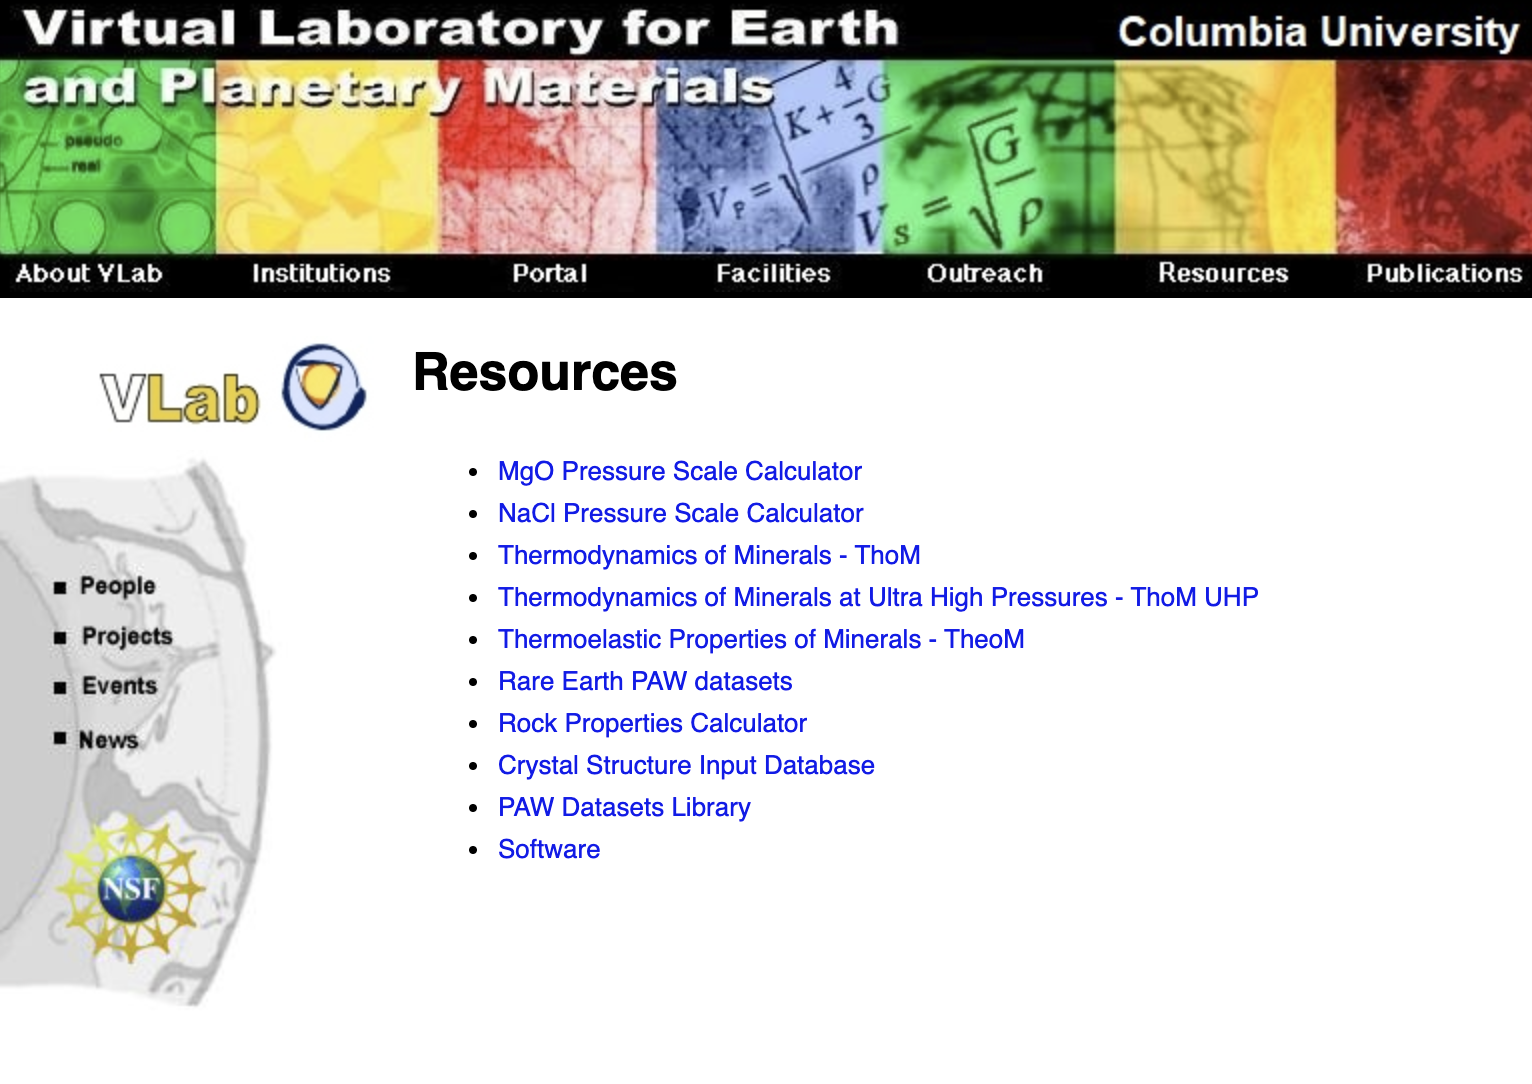
\includegraphics[width=\textwidth]{vlab}};
                \draw (1, 1) node {Hello world};
            \end{tikzpicture}
        \end{column}
    \end{columns}
    \footcitetext{DASILVA2007321}

    \begin{tikzpicture}[overlay, remember picture]
        \node[xshift=-1cm,yshift=-1cm] at (current page.north east) {\qrcode[height=2cm]{http://mineralscloud.com/resources/}};
    \end{tikzpicture}
\end{frame}

% \subsection{Dispatcher and job scheduler}

\begin{frame}{\subsecname}
    The core of \express{} is its dispatching system,
    which is implemented by
    \href{https://github.com/MineralsCloud/SimpleWorkflows.jl}{\texttt{SimpleWorkflows.jl}},
    taking inspiration from
    \href{https://github.com/invenia/Dispatcher.jl}{\texttt{Dispatcher.jl}}
    (currently unmaintained) and
    \href{https://github.com/cihga39871/JobSchedulers.jl}{\texttt{JobSchedulers.jl}}.

    \begin{columns}[t]
        \begin{column}{0.4\textwidth}
            \begin{center}
                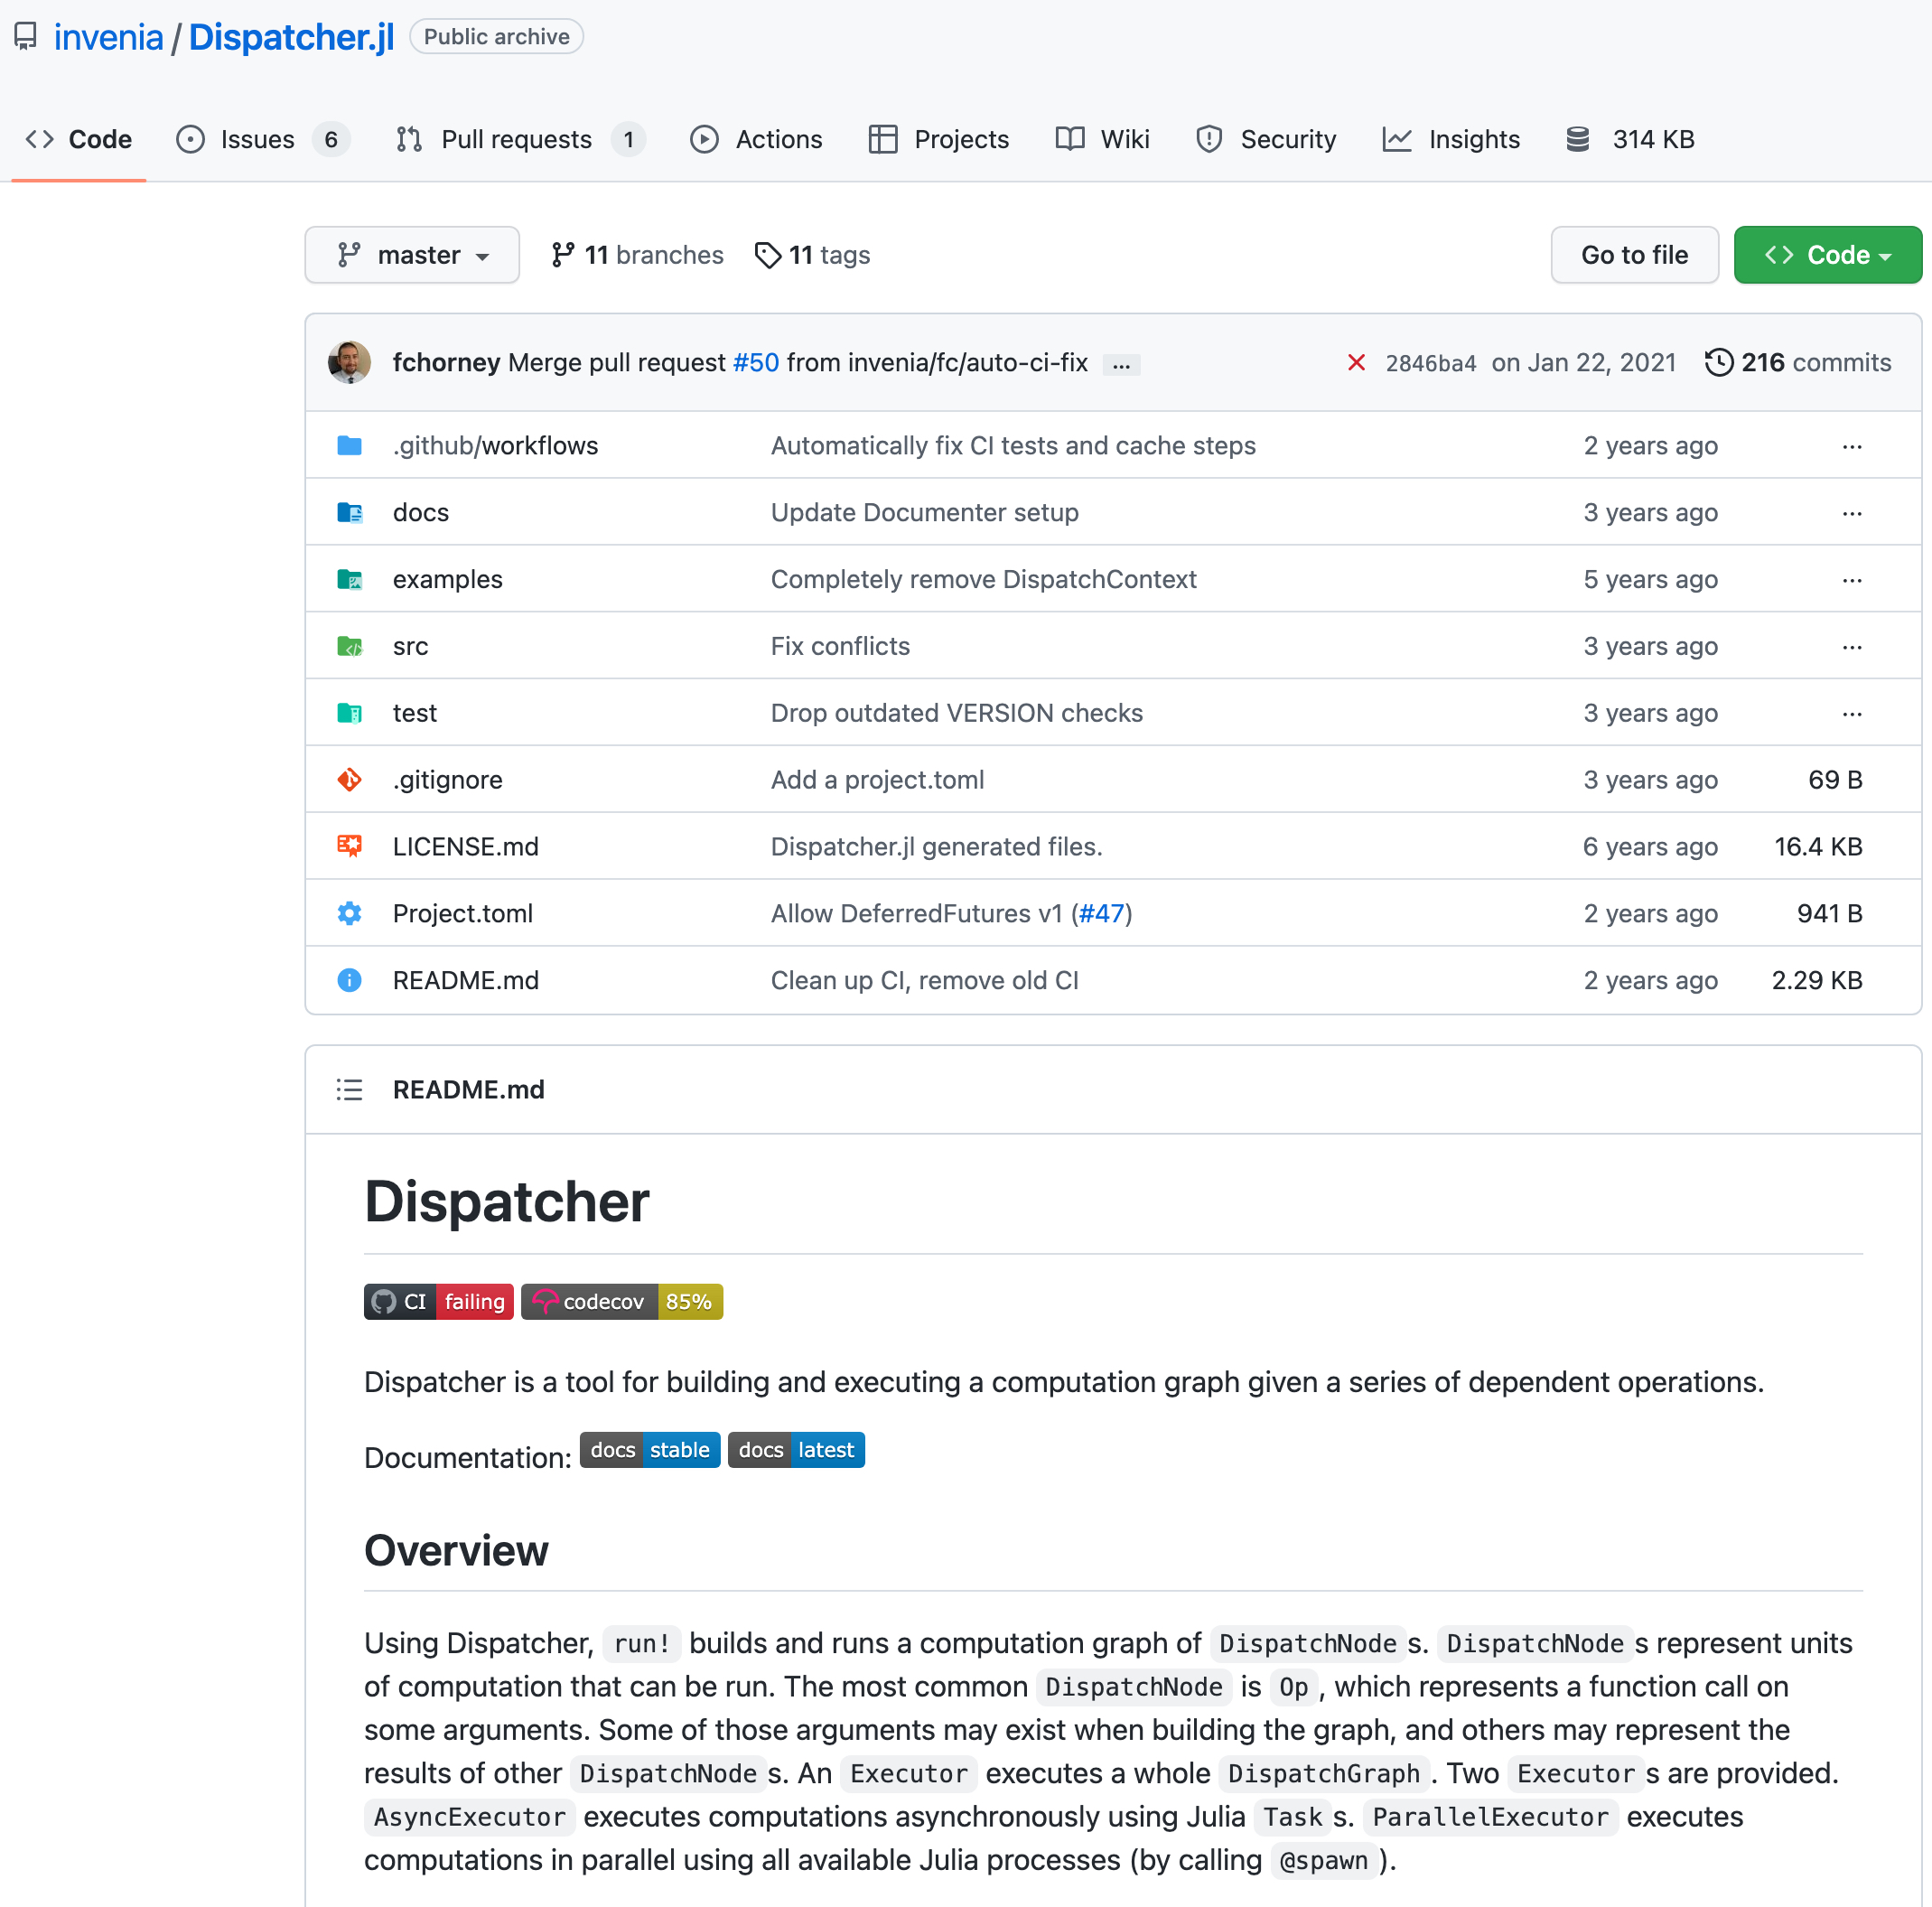
\includegraphics[height=0.5\textheight]{Dispatcher}
            \end{center}
        \end{column}
        \hfill
        \begin{column}{0.4\textwidth}
            \begin{center}
                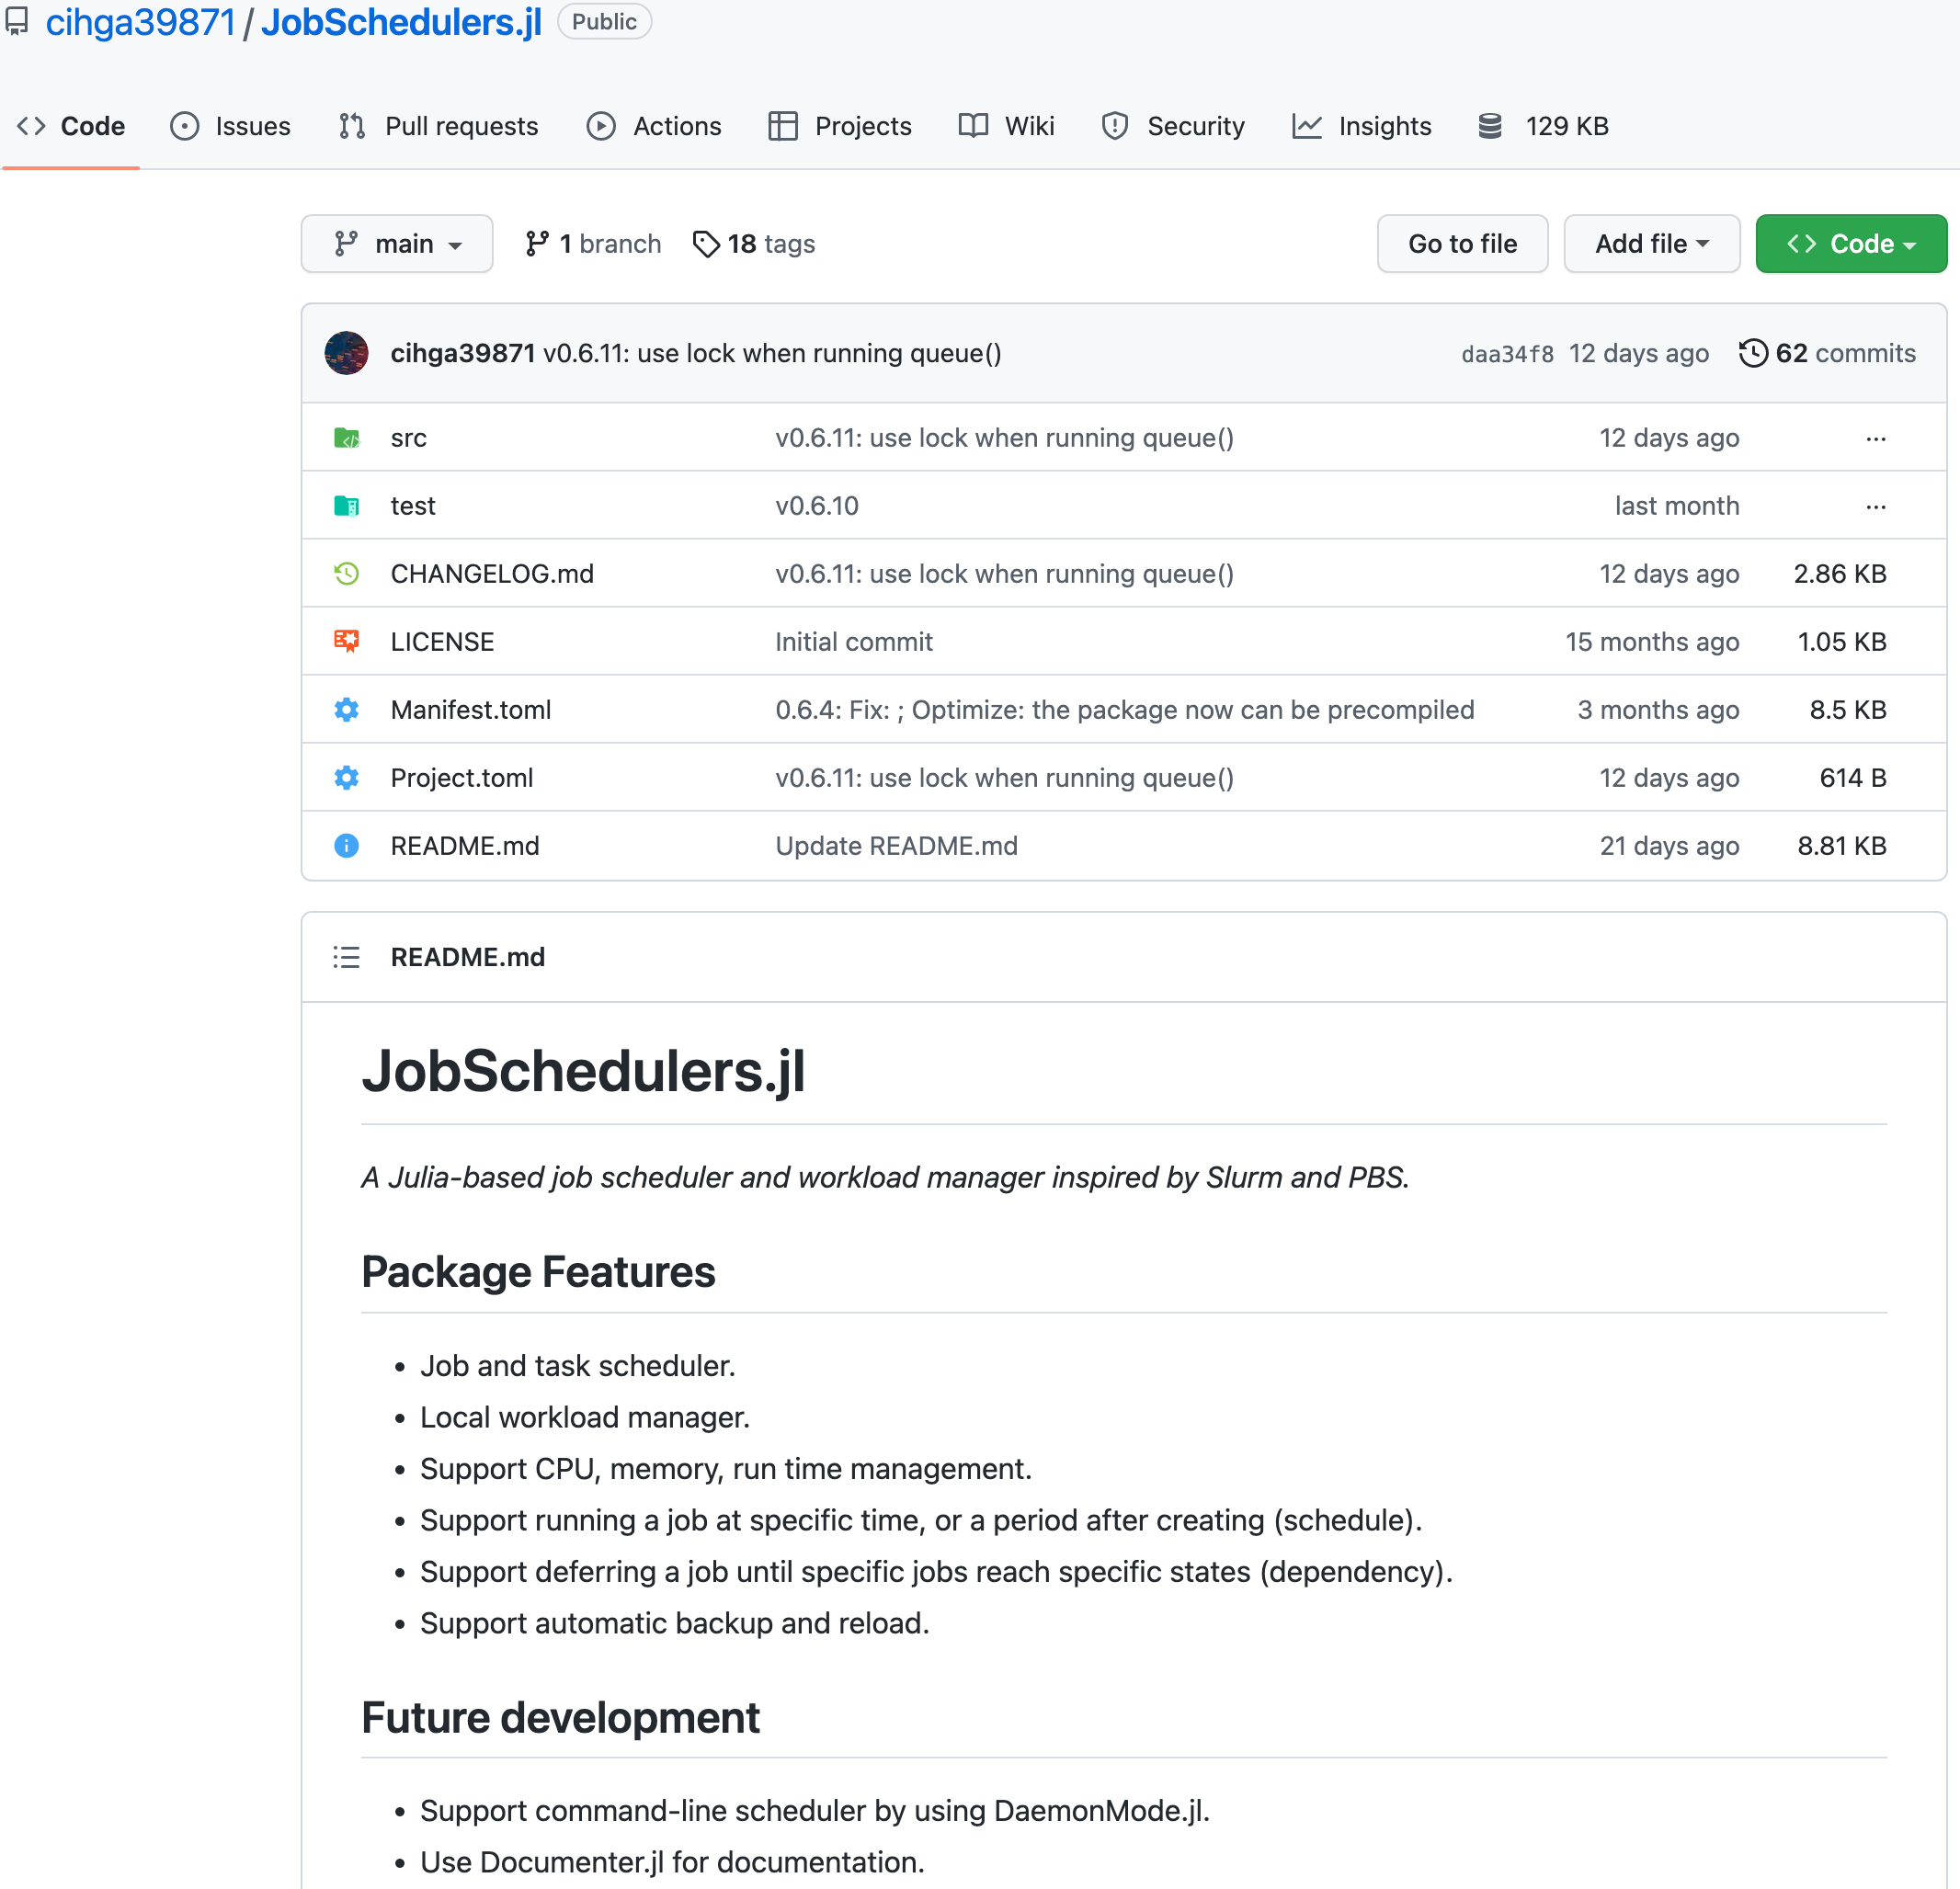
\includegraphics[height=0.5\textheight]{JobSchedulers}
            \end{center}
        \end{column}
    \end{columns}
\end{frame}

\begin{frame}[fragile]
    \frametitle{\subsecname}
    \framesubtitle{Design overview}

    The simplest atomic operation in a \texttt{Workflow} is called a \texttt{Job}.
    It tracks the time, result, and other info of the user's input.
    The relationship between each \texttt{Job} in the \texttt{Workflow} is represented by a
    DAG.\\

    To construct a \texttt{Workflow}, we provide some operators to simplify this step.

        {\footnotesize
            \begin{algorithmblock}
                \begin{juliaverbatim}
using SimpleWorkflows: →, ⇉, ⇶, ↣

a0 → a ⇉ b ⇶ c ↣ d0 → d → f → g ⇉ h ⇶ i ↣ j0 → j → l
        \end{juliaverbatim}
            \end{algorithmblock}
        }
\end{frame}

% [fragile] needed when the content contains juliaverbatim.
\begin{frame}[fragile, allowframebreaks]
    \frametitle{\subsecname}
    \framesubtitle{An example}

    Let's construct an arbitrary \texttt{Workflow}:
    {\scriptsize
    \begin{algorithmblock}
        \begin{juliaverbatim}
using SimpleWorkflows
i = @job (println("Start job `i`!"); sleep(5)) user = "me" desc = "i"
j = @job (println("Start job `j`!"); sleep(3); exp(2)) user = "me" desc = "j"
k = @job (println("Start job `k`!"); sleep(6)) desc = "k"
l = @job (println("Start job `l`!"); run(`sleep 3`)) desc = "l" user = "me"
m = @job (println("Start job `m`!"); sleep(3); sin(1)) desc = "m"
n = @job (println("Start job `n`!"); run(`pwd` & `ls`)) user = "me" desc = "n"
i → l
j → k → m → n
j → l
k → n
wf = Workflow(k)
        \end{juliaverbatim}
    \end{algorithmblock}
    }

    \framebreak

    The DAG of the \texttt{Job}s from \texttt{i} to \texttt{n} is

    \begin{figure}[H]
        \centering
        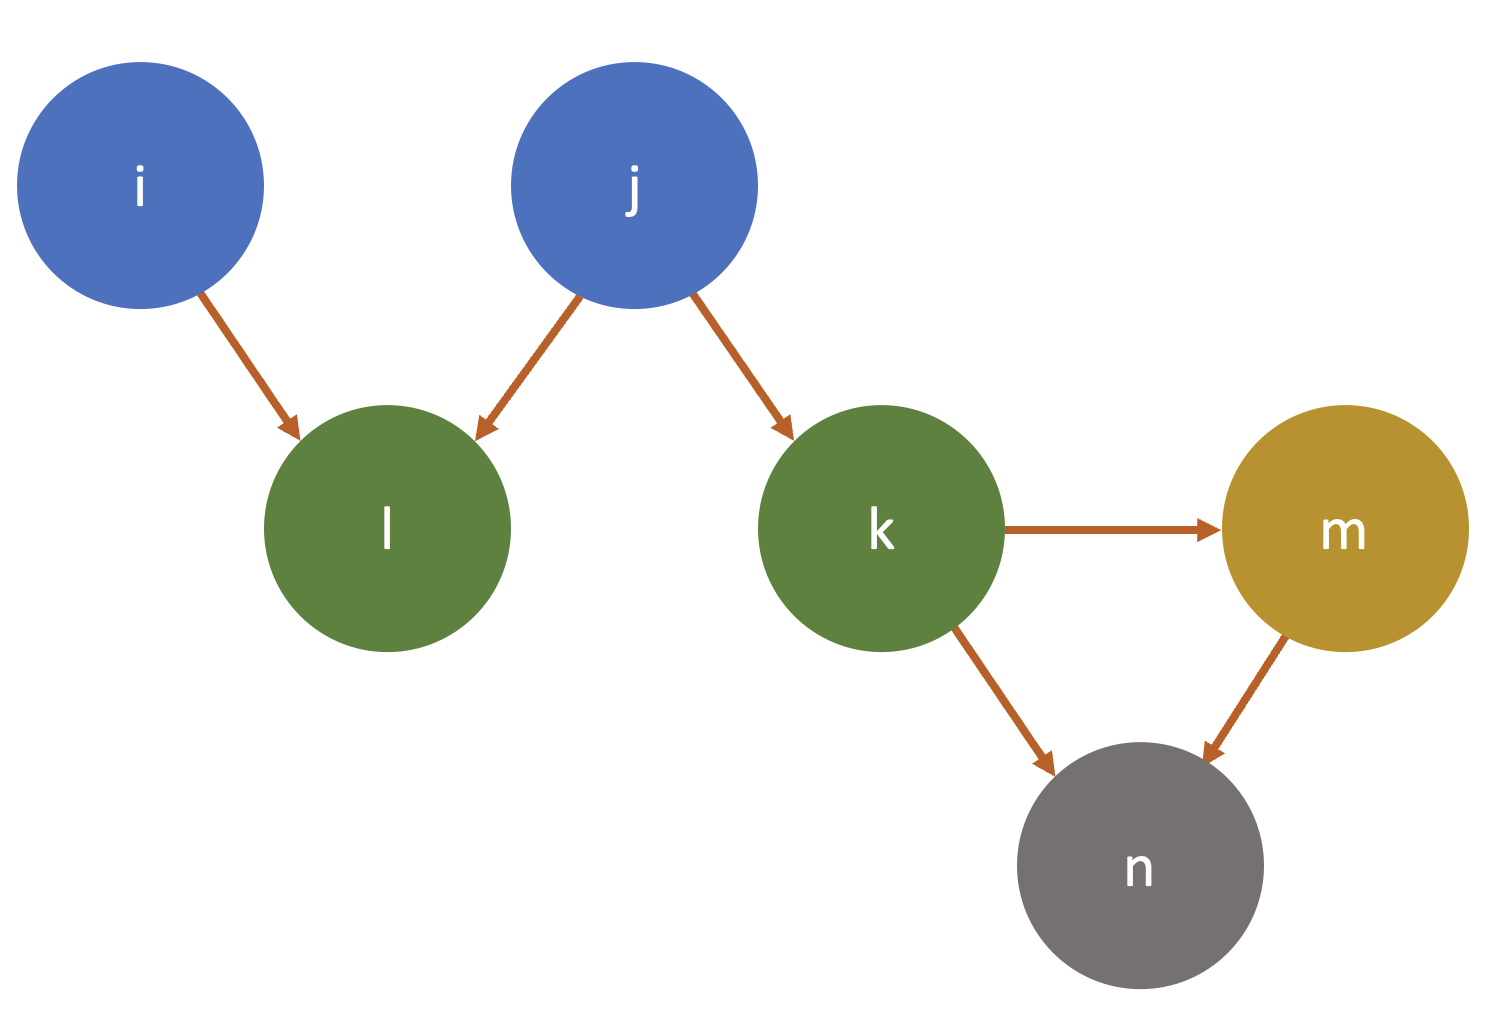
\includegraphics[height=0.35\textheight]{order}
        \caption{The execution order of the \texttt{Job}s from \texttt{i} to \texttt{n}.
            Blue circles are the first, then green, then yellow, and gray is the last.}
        \label{fig:order}
    \end{figure}

    \texttt{Jobs} of the same order are executed in parallel or asynchronously by
    Kahn's algorithm.

    \framebreak

    After or during the execution of the \texttt{Workflow}, we can use \texttt{queue} to
    print all the \texttt{Job}s' information:

    {\scriptsize
    \begin{algorithmblock}
        \begin{juliaverbatim}
run!(wf)
queue()
        \end{juliaverbatim}
    \end{algorithmblock}
    }

    \begin{figure}[H]
        \centering
        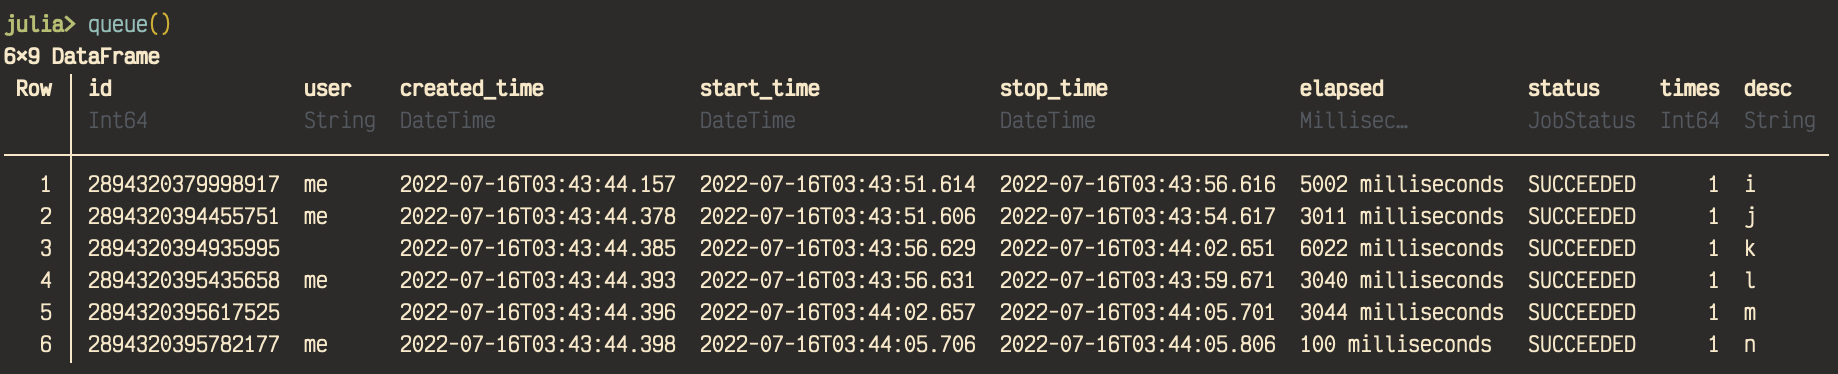
\includegraphics[width=0.8\textwidth]{queue}
        \caption{Queuing the information of the \texttt{Job}s in a \texttt{Workflow}.}
        \label{fig:queue}
    \end{figure}

    And a \texttt{JLD2} format file will be saved during this step. If some errors happen
    during the running or the execution is interrupted, we can rerun only the
    failed/interrupted \texttt{Jobs} according to the information saved in that file.
\end{frame}

% \subsection{User interface}\label{ssec:ui}

\begin{frame}
    \frametitle{\subsecname}
    \framesubtitle{Motivation}

    \begin{block}{What should be the most commonly-used interface}
        Since most tasks in different \ab{} calculations are routine, with only
        input parameters changed. It is desirable to make an interface that takes a few
        parameters each time.

        A command line interface plus a template file for the \ab{} software for the sciency
        fixed settings and a configuration file for the computational variables is a
        balanced choice.
    \end{block}

    \begin{block}{Command line interface}
        We want a command line interface to have

        \begin{itemize}
            \item A single topmost command (\texttt{xps})
            \item A few second-tier commands corresponding to different workflows
            \item A few third-tier commands corresponding to different tasks in a workflow
            \item A few arguments, flags, and options for each command mentioned above
        \end{itemize}
    \end{block}
\end{frame}

% [fragile] needed when the content contains juliaverbatim.
\begin{frame}[fragile, allowframebreaks]
    \frametitle{\subsecname}
    \framesubtitle{Implementation}

    With \href{https://github.com/comonicon/Comonicon.jl}{\texttt{Comonicon.jl}}, we can implement
    an aforementioned interface easily.

        {\scriptsize
            \begin{algorithmblock}
                \begin{juliaverbatim}
module ExpressCommands
using Comonicon: @cast, @main

@cast function print(file)
    ...
end

@main
end
                \end{juliaverbatim}
            \end{algorithmblock}
        }

    Then we can run

        {\scriptsize
            \begin{algorithmblock}
                xps print config.toml
            \end{algorithmblock}
        }

    to print a configuration file, for example.

    \framebreak

    To build subcommands for different workflows, we use modules inside the global module
    (\texttt{ExpressCommands}) to do that:

    {\scriptsize
    \begin{algorithmblock}
        \begin{juliaverbatim}
module ExpressCommands

module EOS

using Comonicon: @cast

@cast function fit(calc, cfgfile)
    ...
end

end

end
        \end{juliaverbatim}
    \end{algorithmblock}
    }

    See package \texttt{ExpressCommands.jl} for more details.
\end{frame}

\begin{frame}
    \frametitle{\subsecname}
    \framesubtitle{Run commands with configuration files}

    \begin{columns}[t]
        \begin{column}{0.4\textwidth}
            As stated in previous slides, we could put computational settings
            in a configuration file to change variables dynamically.

            We make use of
            \href{https://github.com/Roger-luo/Configurations.jl}{\texttt{Configurations.jl}},
            which can read TOML files into a Julia \texttt{struct}
            (similar to \href{https://github.com/quinnj/JSON3.jl}{\texttt{JSON3.jl}}).
            We accept JSON and YAML formats as well.

            A typical configuration file looks like this (items may change in the future versions):
        \end{column}

        \begin{column}{0.6\textwidth}
            \begin{minted}[frame=single, linenos]{toml}
            recipe = "eos"
            template = "template.in"
            [cli.mpi]
            np = 128
            [save]
            status = "status.jls"
            eos = "eos.jls"
            [trial_eos]
            type = "bm3"
            values = ["300.44 bohr^3", "74.88 GPa", 4.82]
            [fixed.pressures]
            unit = "GPa"
            values = [-5, -2, 0, 5, 10, 15, 17, 20]
        \end{minted}
        \end{column}
    \end{columns}

\end{frame}


\section{What is an \ab{} workflow system?}

\subsection{What are \ab{} calculations?}

\begin{frame}{What are \ab{} calculations?}
    \begin{definitionblock}{\ab{} calculation}
        A method of calculating atomic and molecular structure directly from the first
        principles of quantum mechanics, without using quantities derived from experiment
        as parameters.
    \end{definitionblock}

    \begin{itemize}
        \item Electronic structure computation
        \item Optimize input crystal/molecular structures
        \item Phonon vibrational spectra computation
        \item Helmholtz free energy calculation at finite temperature
        \item Linear elastic constants
        \item More...
    \end{itemize}
\end{frame}

\begin{frame}{Typical \ab{} workflows used in our group}
    \begin{figure}[H]
        \centering
        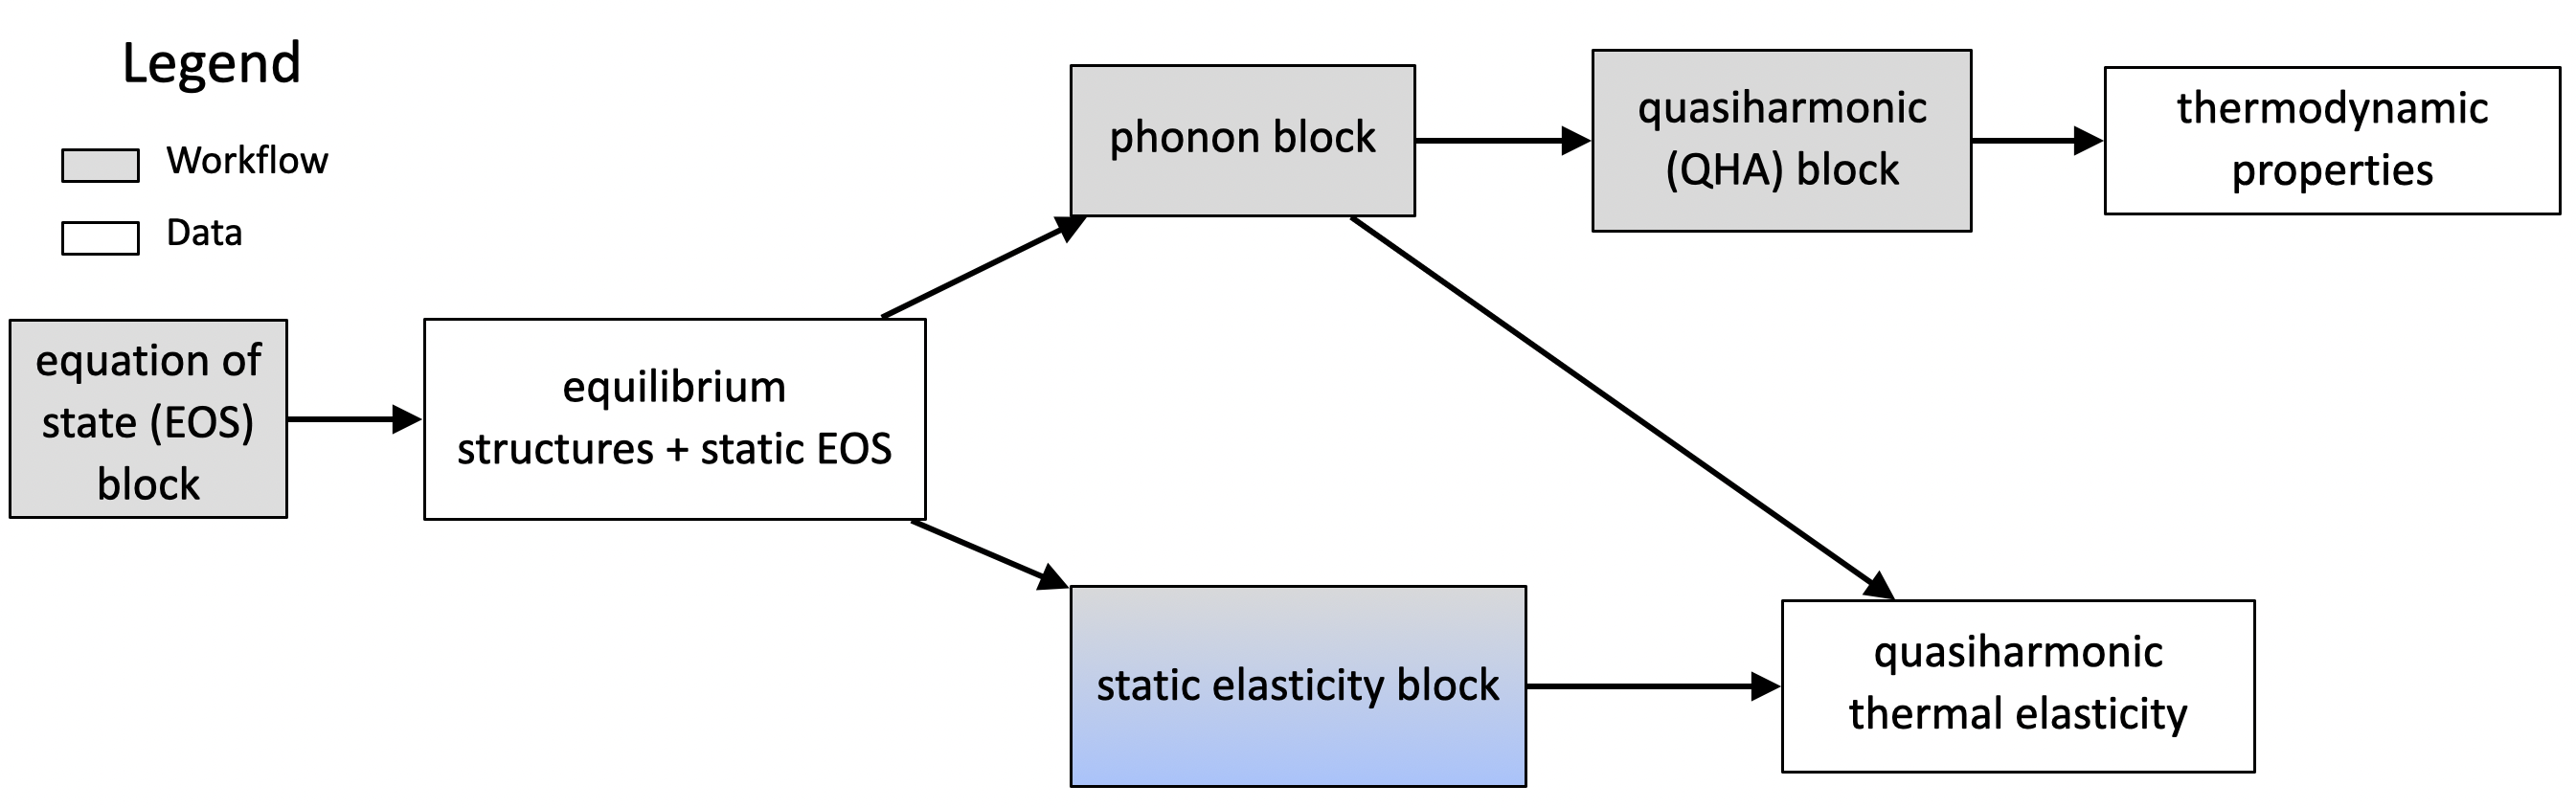
\includegraphics[height=0.4\textheight]{workflows}
        \label{eq:workflows}
    \end{figure}
\end{frame}

\begin{frame}{Various \ab{} software}
    To do \ab{} calculations, it is inevitable to interact with \ab{} software.
    There are a lot of them on the market, e.g., \qe{}, VASP, and ABINIT.
    They are often written in Fortran, and needed to be compiled to executable
    when using.

    So building a workflow for them requires us to create parsers for their input and output
    files, as well as functions to dynamically run these executables.

    \begin{figure}[b]
        \centering
        
\includegraphics[width=0.4\textwidth]{qe}
        \hfill
        
\includegraphics[width=0.2\textwidth]{vasp}
        \hfill
        
\includegraphics[width=0.3\textwidth]{abinit}
        \label{fig:abinitsoftware}
    \end{figure}
\end{frame}
\subsection{What is needed in an \ab{} workflow system?}

\begin{frame}{What is needed in an \ab{} workflow system?}
    There are at least three components:

    \begin{itemize}
        \item Sciency, technical stuff: calculations, input generation, output analysis...
        \item Dispatcher, job scheduler: interacting with \ab{} software, \texttt{mpi}...
        \item User interface: interacting with users
    \end{itemize}
\end{frame}

\subsection{What does \express{} do?}

\begin{frame}{What does \express{} do?}
    A Julia-written
    \begin{itemize}
        \item extensible,
        \item lightweight,
        \item high-throughput,
        \item high-level
    \end{itemize}
    workflow framework that aims to automate \ab{} calculations for the materials science
    community.
\end{frame}

\section{How to build an \ab{} workflow system}

\subsection{Sciency, technical stuff}

\subsubsection{Binary dependencies \& foreign function interface}

\begin{frame}
    \frametitle{\subsubsecname}
    \framesubtitle{Building an artifact}

    Operations like finding the symmetry of a crystal
    are very common in \ab{} calculations (usually the first step).
    Therefore, we need a good library to do this.

    There is a C library called \href{https://github.com/spglib/spglib}{\texttt{spglib}}
    that does this.
    To make it a productive library, we need first put it in a container
    (``artifacts''). Luckily, the amazing Julia community has made it possible:
    \href{https://github.com/JuliaBinaryWrappers/spglib_jll.jl}{\texttt{spglib_jll.jl}}.
\end{frame}

\begin{frame}[fragile]
    \frametitle{\subsubsecname}
    \framesubtitle{Foreign function interface}

    \begin{columns}
        \begin{column}{0.3\textwidth}
            Now that we have an artifact that exports the functions of the C library,
            it may still be hard to use since it uses some C data structures and API, which may
            not be idiomatic in Julia. Therefore, we need to wrap it with a higher level of APIs.
            \href{https://github.com/singularitti/Spglib.jl}{\texttt{Spglib.jl}} is built based on
            this expectation.
        \end{column}

        \begin{column}{0.7\textwidth}
            {\tiny
                \begin{algorithmblock}
                    \begin{juliaverbatim}
function standardize_cell(
    cell::Cell;  # `Cell` was not defined in the C library
    to_primitive = false,
    no_idealize = false,
    symprec = 1e-5,
)
    @unpack lattice, positions, types = _expand_cell(cell)
    to_primitive = Base.cconvert(Cint, to_primitive)
    no_idealize = Base.cconvert(Cint, no_idealize)
    num_atom = Base.cconvert(Cint, length(types))
    allocations = 4
    _positions = Matrix{Cdouble}(undef, 3, num_atom * allocations)
    _types = Vector{Cint}(undef, num_atom * allocations)
    _positions[:, 1:num_atom] = positions
    _types[1:num_atom] = types
    n = ccall(
        (:spg_standardize_cell, libsymspg),
        Cint,
        (Ptr{Cdouble}, Ptr{Cdouble}, Ptr{Cint}, Cint, Cint, Cint, Cdouble),
        lattice,
        _positions,
        _types,
        num_atom,
        to_primitive,
        no_idealize,
        symprec,
    )
    return Cell(transpose(lattice), _positions[:, 1:n], _types[1:n])
end
                    \end{juliaverbatim}
                \end{algorithmblock}
            }
        \end{column}
    \end{columns}
\end{frame}

\subsubsection{Parsers for \ab{} software I/O}

\begin{frame}[allowframebreaks]{\subsubsecname}
    Most \ab{} software is written in Fortran and has plain text files as input \& output.
    Therefore, we need parsers for both of them. But it is tricky...

        {\footnotesize
            \begin{itemize}
                \item For example, \qe{}'s input adopts the \texttt{Namelist} data structure from
                      Fortran. Julia does not have a parser for Fortran...
                \item A Python package
                      (\href{https://github.com/marshallward/f90nml}{\texttt{f90nml}}) can do that.
                      I wrote a very preliminary package
                      \href{https://github.com/singularitti/PyFortran90Namelists.jl}{\texttt{PyFortran90Namelists.jl}},
                      to call that Python code.
                \item However, it uses \texttt{PyCall.jl}, so sometimes people have trouble installing
                      it if they already have Python installed
                      (see \href{https://github.com/JuliaPy/PyCall.jl\#specifying-the-python-version}{``Specifying the Python version''}).
            \end{itemize}
        }

    For output files, it is even more complicated since they usually do not have a standard
    format. Therefore lots of regular expressions need to be used.
    It is extremely error-prone. I used
    \href{https://github.com/jkrumbiegel/ReadableRegex.jl}{\texttt{ReadableRegex.jl}} to build them.
\end{frame}

\subsubsection{A wrapper for \ab{} software executables}

\begin{frame}[fragile, allowframebreaks]{\subsubsecname}
    To run external \ab{} software within Julia, what should we do?\\

    Use the Julia \texttt{AbstractCmd}s? Good choice!
    But sometimes, we want to generate a series of \texttt{AbstractCmd}s dynamically,
    especially in a workflow system.
    Writing them one by one is not so efficient.\\

    Wait, can we write functions to generate \texttt{AbstractCmd}s? Then all the command
    arguments will be standard Julia function arguments! For example,

    {\scriptsize
            \begin{algorithmblock}
                \begin{juliaverbatim}
mpirun -np 16 pw.x -npool 2 -nk 2 -input scf_in > scf_out
                \end{juliaverbatim}
            \end{algorithmblock}
        }

    will be

        {\scriptsize
            \begin{algorithmblock}
                \begin{juliaverbatim}
pw("scf_in", "scf_out"; np = 16, npool = 2, nk = 2)
                \end{juliaverbatim}
            \end{algorithmblock}
        }

    \framebreak

    What's more, we could use
    \href{https://github.com/comonicon/Comonicon.jl}{\texttt{Comonicon.jl}},
    to build new executables that will provide customized arguments
    (see \href{https://github.com/MineralsCloud/QuantumESPRESSOCommands.jl}{\texttt{QuantumESPRESSOCommands.jl}})

    {\scriptsize
            \begin{algorithmblock}
                \begin{juliaverbatim}
using Comonicon: @cast
@cast function pw(input, output = mktemp(parentdir(input))[1];
                  np = 1, npool = 1, nk = 1, path = "pw.x", chdir = false)
    ...
    return run(cmd)
end
                \end{juliaverbatim}
            \end{algorithmblock}
        }

    Therefore, we could run it with

        {\scriptsize
            \begin{algorithmblock}
                \begin{juliaverbatim}
pw -np 16 -npool 2 -nk 2 -input scf_in scf_out
            \end{juliaverbatim}
            \end{algorithmblock}
        }

\end{frame}


\begin{frame}{Acknowledgments}
    This work was supported by DOE award DE-SC0019759. It used the Extreme
    Science and Engineering Discovery Environment (XSEDE), which is supported by
    the National Science Foundation grant number ACI-1548562 and allocation
    TG-DMR180081.\\

    The authors also thank Jiayang Wang, Michel Marcondes, Hongjin Wang, and Pedro da Silveira
    for their contributions and suggestions to this code.\\

    Please cite our work as:

    \cite{zhang2021textttexpress}.
\end{frame}

% See https://tex.stackexchange.com/a/215059/61591
\begin{frame}[c]
    \centering \fontsize{40}{50}\selectfont\emph{Thank You!}
\end{frame}



\begin{frame}{References}
    \printbibliography
\end{frame}

\end{document}
